\subsection{Luftflöde genom väggar – drag}
\label{sec:leakagewall}

När det blåser på fastigheten får det luften kring fastigheten att cirkulera och även tränga in i 
byggnaden. När vinden ligger på med $\unit[3]{m~s^{-1}}$, vinkelrätt mot nord- eller sydfasaden fås 
ett flöde som det i figur~\ref{fig:windspeed} och trycket som då uppstår visas i figur~
\ref{fig:windpressure}. Tryckskillnaderna på de olika sidorna av husen kommer att driva 
ofrivillig ventilation vilket leder till energiförluster i form av infiltration.

\begin{figure}[hpbt]
\centering
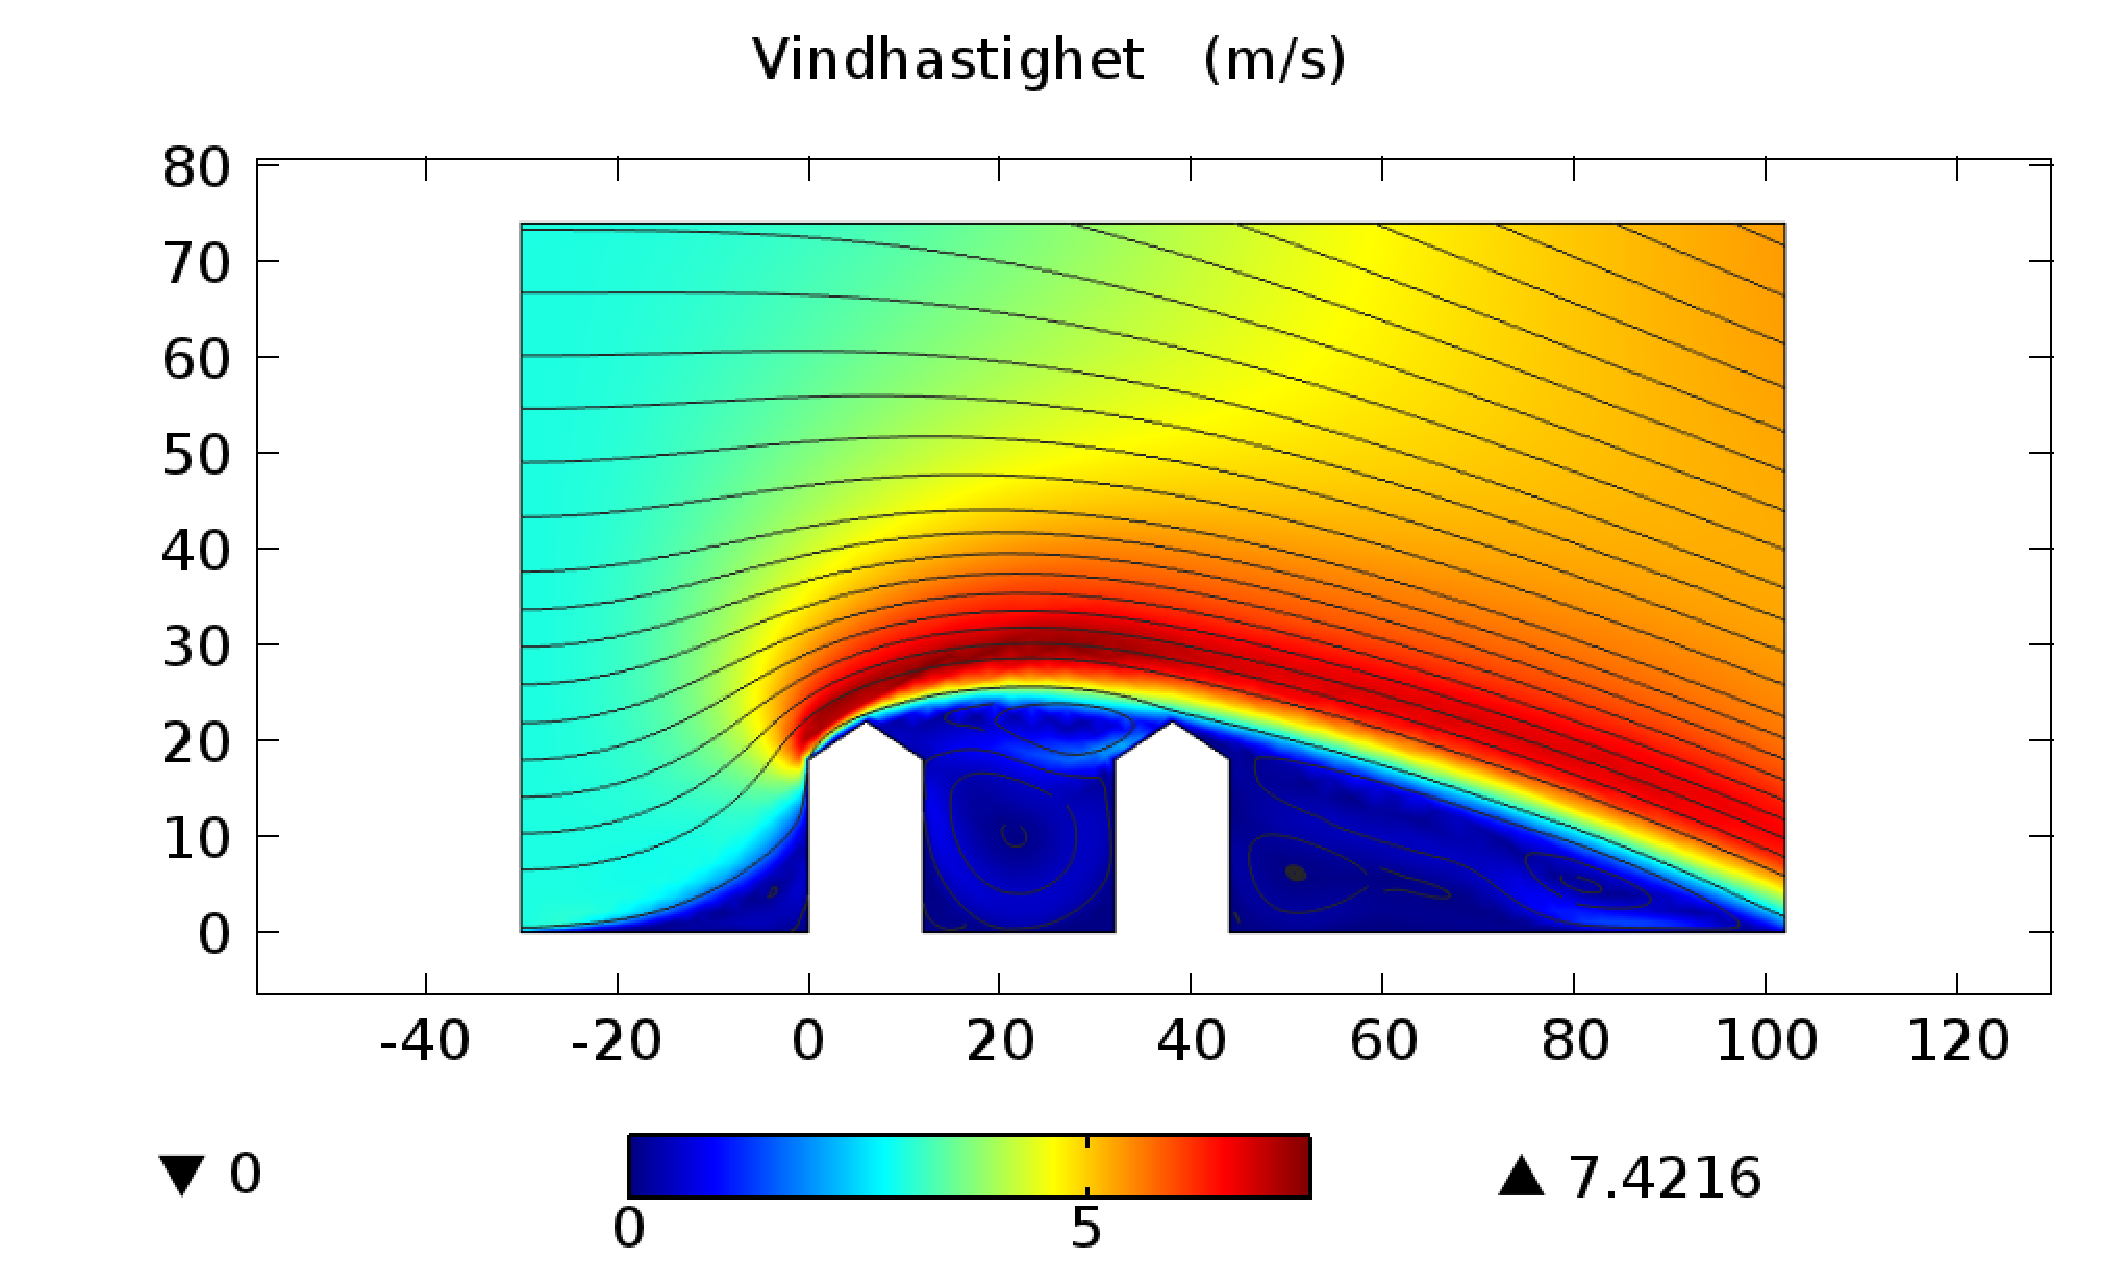
\includegraphics[width=127mm,height=76mm]{images/wind3mshdpi.eps}
\caption{\label{fig:windspeed}Vindhastiheten när vind i $\unit[3]{m~s^{-1}}$ blåser mot fastigheten 
från vänster sida i figuren. Linjerna är strömlinjer och färgen indikerar farten. Värdena är 
framräknade med Comsol. Enhet $\unit{m~s^{-1}}$.}
\end{figure}


\begin{figure}[hpbt]
\centering
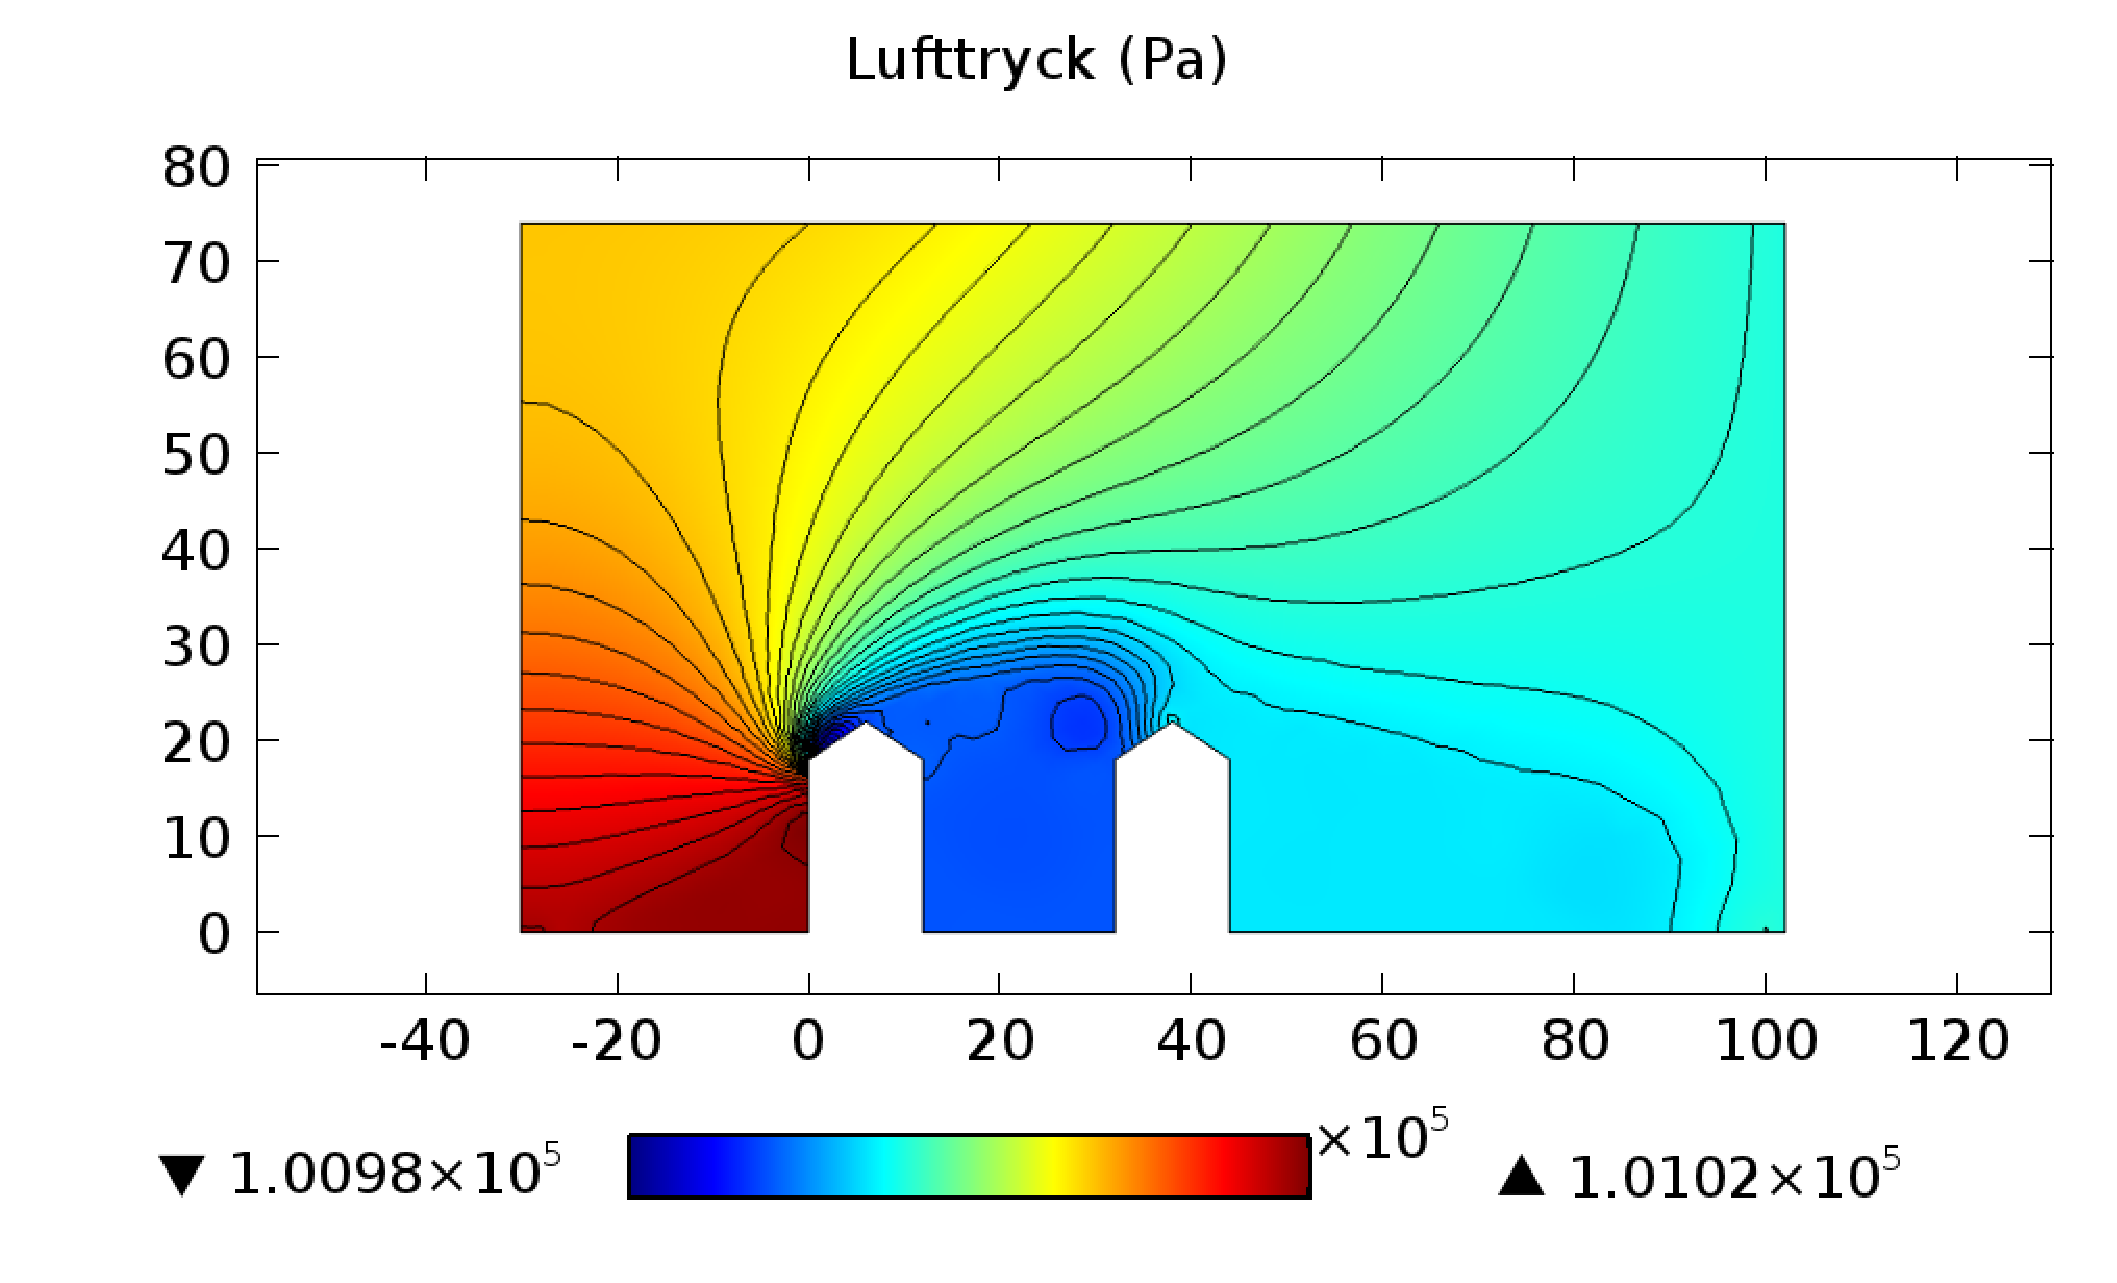
\includegraphics[width=127mm,height=76mm]{images/pressure3mshdpi.eps}

\caption{\label{fig:windpressure}Lufttrycket när vind i $\unit[3]{m~s^{-1}}$ blåser mot fastigheten från vänster sida i figuren. Linjerna är isobarer, färgen indikerar lufttryck. Värdena är framräknade med Comsol. Enhet Pa.}
\end{figure}

% Resultat
Ur figur~\ref{fig:windspeed} fås att det hus som ligger i lä inte utsätts för någon vind att tala om.
 Vidare fås ur figur~\ref{fig:windpressure} att huset i lä utsätts för en betydligt mindre 
 tryckskillnad, än den byggnad som det blåser direkt på. I vårt exempel här, med en 
 vindhastighet omring $\unit[3]{m~s^{-1}}$ fås en maximal tryckskillnad mellan norr- och sydväggarna.
 på 40 Pa, för fastigheten i lovart. Tryckskillnaden ökar med stigande vindhastighet och vid $\unit[10]{m~s^{-1}}$ fås en 
 tryckskillnad på $\unit[340]{Pa}$ för fastigheten i lovart. 

Applicerat på fastigheten på Walleriusgatan betyder detta att sydvindar ger upphov till 
betydligt mer infiltrationsförluster än nordvindar. Till den aktuella byggnadens fördel ska nämnas 
att södervindarna ofta är varmare än nordvindarna och de faktiska energiförlusterna 
troligen blir något mindre.

%%%%%%%%%%%%%%%%%%%%%%%%%%%%%%%%%%%%%%%%

Energiförlusterna på grund av drag har beräknats utifrån att en bestämd mängd energi per grad finns lagrad i en viss volym luft. Luftflödet genom väggen har beräknats på flera sätt, både med Darcys lag och med byggfysikformeln, se avsnitt~\ref{subsec:darcy}.

Energiförlusten har beräknats
  för en fastighet i lovart respektive en som ligger i lä av en annan byggnad, precis som 
  byggnaderna i figur~\ref{fig:windspeed} och \ref{fig:windpressure}, vilket motsvarar att det 
  blåser på fastigheten på Walleriusgatan från söder respektive norr. Resultatet kan ses i figur~
  \ref{fig:windenergyloss} för en byggnad i lovart och en i lä samt för ett teoretiskt framtaget hus. Dessa två olika kurvor, framtagna med Darcys lag samt med byggfysikformeln, får motsvara högsta respektive minsta gissningar för infiltrationsförluster i en byggnad. \emph{\color{red} Vad representerar den teoretiska huset? Vad vill vi säga med det?}

Trycken i figur~\ref{fig:windenergylossa} och \ref{fig:windenergylossb} är framräknade för 
olika vindhastigheter med programmet Comsol medan den teoretiska modellen i figur~
\ref{fig:windenergylossc} är beräknad med med en approximation. 

Approximationen\emph{\color{red} Vilken approximation} baserar sig på att tryckskillnaden mellan inne och ute är proportionerligt mot vindhastigheten i kvadrat. Denna visar hur kyleffekten blir på en fristående rätblocksformad byggnad. Den exakta kyleffekten beror till stor del på vilken omgivning byggnaden står i. \emph{\color{red} Denna förklaring på teoretiska huset är tunn och förvirrad.}


\begin{figure}[hpbt]
\centering
\subfloat[\label{fig:windenergylossa}Byggnad som vinden blåser direkt på.]{
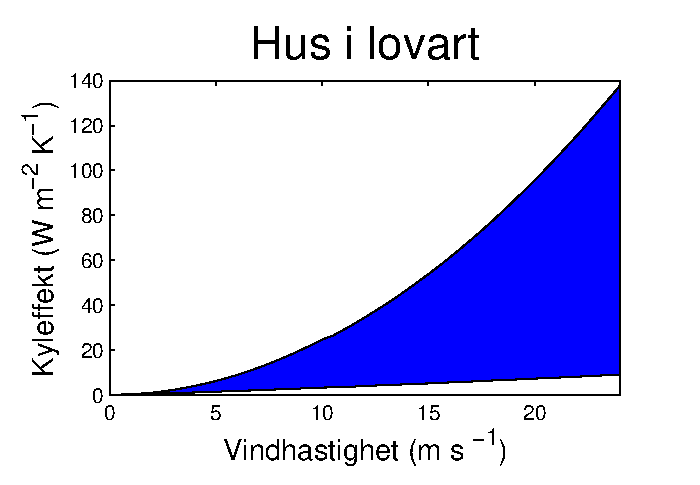
\includegraphics[width=60mm]{images/pressurewind.eps}}
\vspace{5mm}
\subfloat[\label{fig:windenergylossb}Byggnad som ligger i lä av en annan byggnad.]{
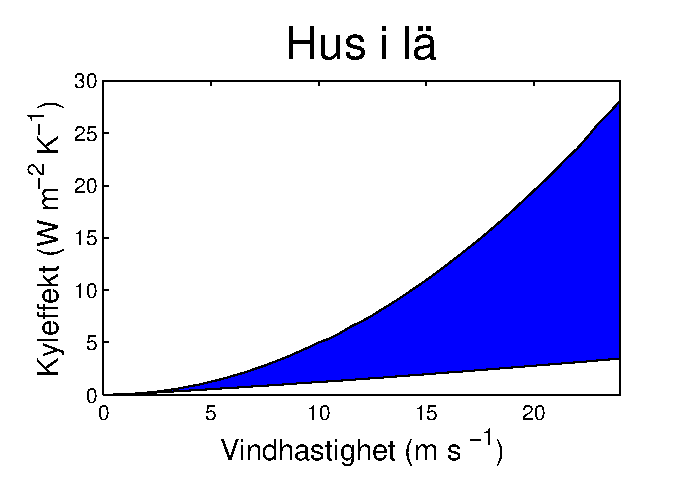
\includegraphics[width=60mm]{images/pressurenowind.eps}}

\subfloat[\label{fig:windenergylossc}Teoretisk approximation för lådformad byggnad.]{
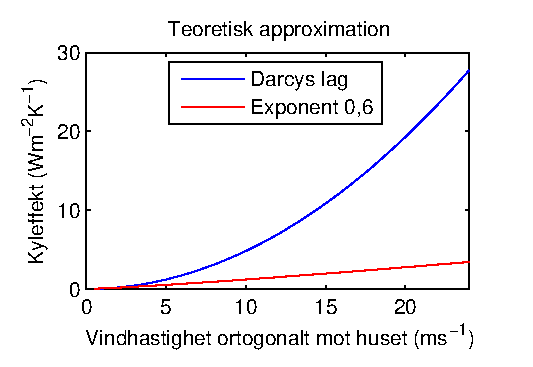
\includegraphics[width=60mm]{images/pressuretheory.eps}}

\caption{\label{fig:windenergyloss}Energiförlust per grad, max- respektive minvärde.
Framtaget med Comsol (a och b) och teoretiskt framräknade med en approximation (c).}
\end{figure}

% Resultat
Vilken kyleffekt vinden har på fastigheten är mer osäkert vid högre vindhastigheter. När vinden
 ligger på med uppemot $\unit[25]{m~s^{-1}}$ kan kyleffekten variera från några tiotal $\unit{W~m^{-2}~K^{-1}}$ upp 
 emot drygt 100. Motsvarande kan kyleffekt för ett hus i lä vara mellan några $\unit{W~m^{-2}~K^{-1}}$ upp mot knappt 30. För det teoretiskt beräknade huset fås även där att kyleffekten 
 kan vara mellan några $\unit{W~m^{-2}~K^{-1}}$ upp mot knappt 30 $\unit{W~m^{-2}~K^{-1}}$. När vi har mer normala $\unit[10]{m~s^{-1}}$ ser vi istället att kyleffekten kan vara från några få upp emot $\unit[20]{W~m^{-2}~K^{-1}}$ för en byggnad i 
 lovart, och ungefär en fjärdedel av det för en byggnad i lä.
 
För fastighetens norrvägg, den som ligger i lä av en annan fastighet, fås infiltrationsförluster upp till $\unit[28]{kW}$ vid $\unit[10]{m~s^{-1}}$ och temperaturen $\unit[5]{^\circ C}$, då den har arean $\unit[379]{m^2}$. För söderväggen, som ligger mer fritt och har arean $\unit[307]{m^2}$ fås förluster upp till $\unit[115]{kW}$ vid samma vindhastighet. Detta är med beräkningar ur Darcys lag vilket kan anses vara extremt högt räknat och det är mycket otroligt att huset läcker så mycket.

